% \documentclass[submit,techreq,noauthor]{eco}	% semi style
\documentclass[submit,techreq,noauthor,dvipdfmx]{mid-eco}
\usepackage[dvips]{graphicx}
\usepackage{listings, jlisting} 		% for source code
\usepackage{url}
\usepackage{setspace}
\usepackage{here}
%\setstretch{1.5} % 行間を広くします(資料チェックしてもらうときはコメントを外す)

\lstset{
  basicstyle={\ttfamily},
  identifierstyle={\small},
  commentstyle={\smallitshape},
  keywordstyle={\small\bfseries},
  ndkeywordstyle={\small},
  stringstyle={\small\ttfamily},
  frame={tb},
  breaklines=true,
  columns=[l]{fullflexible},
  numbers=left,
  xrightmargin=0zw,
  xleftmargin=3zw,
  numberstyle={\scriptsize},
  stepnumber=1,
  numbersep=1zw,
  lineskip=-0.5ex
}

\begin{document}

\semino {5/3}					% 年度/回数
\date   {5/07/18/火}				% 平成/月/日/曜日
\title  {LinuxにおけるDynamic Linker Hijacking\\対策のための動的リンカの設計調査}	% タイトル
\author {奥 若菜}				% 氏名


\begin{abstract}
	Linuxマシンが製品やサービスの基盤として広く利用されるようになったことで,それを標的とするLinuxマルウェアが劇的に増加している.
  近年は,Linuxマルウェアの検知回避技術が向上しており,2021年に発見されたマルウェアSymbioteは,極めて検出が困難とされる.
  SymbioteはLD\_PRELOADを使用して,すべての実行中のプロセスにロードされる共有ライブラリとして動作し,
  正当なプロセスの下で自身や他のマルウェアの痕跡を隠蔽する.
  このように,動的リンカの機能を利用して,悪意のある共有ライブラリをプロセスにロードさせる攻撃をDynamic Linker Hijackingという.
  本校では,動的リンカに着目して,マルウェアの検知を困難にするDynamic Linker Hijackingの対策を検討する.
  また,対策を検討する上で,動的リンカの詳細な設計を明らかにする.今回は,実行ファイル実行における動的リンカの動作範囲の特定と,動的リンカのシンボル解決に対する調査を行った.
\end{abstract}
\maketitle


\section{はじめに}
IoTデバイスの普及や組織のクラウドシフトにより,製品やサービスの基盤として,Linuxマシンを利用するケースが増えた.
攻撃対象が広がったことで,それを標的とするLinuxマルウェアも劇的に増加している.AV-ATLASのマルウェアの統計データによると,
TEST}.
Linuxマルウェアの開発動向としては,マルウェアが自身の攻撃をセキュリティソフトに検知されないようにする回避技術の大幅な向上が確認されている\cite{IBM}.
2021年に発見されたSymbioteは,極めて検出が困難とされる\cite{Symbiote}.
Symbioteは,動的リンカによって実行中のプログラムにロードされる共有ライブラリとして動作する.
LD\_PRELOADという環境変数を利用し,Symbioteの共有ライブラリを優先してロードさせることで,本来使用されるライブラリ関数を置き換える.
Symbioteの検出が困難な理由として,ライブラリ関数の置き換えによって,正常なプロセスのもとで任意のファイルやプロセス,通信の隠蔽と改ざんが可能になることがある.
このように,動的リンカの機能を利用して,悪意のある共有ライブラリをプロセスにロードさせる攻撃をDynamic Linker Hijackingといい,この攻撃はマルウェアの検知を困難にする.
%Linuxマルウェアの技術革新の水準はWindowsベースのマルウェアに迫る勢いとされ,この傾向は2022も高まると予想されている.
% このことから,今後もより高度な潜伏機能を持つマルウェアが開発される可能性が高く,対策を怠ると重大な被害に繋がるおそれがある.

Dynamic Linker Hijackingの対策として,動的リンカに関する環境変数や設定ファイルの変更を監視することが提案されている\cite{MITRE-ATT&CK}.
この対策の目的は,攻撃者によって,マルウェアの共有ライブラリをプログラムにロードする設定に変更されることを防ぐことである.
一方で,この設定が行われた場合に,動的リンクの段階で,マルウェアの共有ライブラリのロードを防ぐための対策は考慮されていない.
本稿では,共有ライブラリのロードを行う動的リンカに着目し,動的リンクの段階におけるDynamic Linker Hijackingへの対策を検討する.
また,検討を行うために,Linux動的リンカの詳細な仕様と内部設計を明らかにする.

% Dynamic Linker Hijackingは,マルウェアの検知を非常に困難にする.
%正当なプロセスの下で,マルウェアのコードが実行されるため,プロセスベースの解析は回避される可能性が高い.

以下,2章でLinux動的リンカの調査ついて述べ,3章で実行ファイル実行処理における動的リンカの動作範囲について述べる.
4章で動的リンカのシンボル解決について述べ,5章でまとめる.\\

\section{Linux動的リンカの調査}
\subsection{調査方法}
Linux動的リンカはGNU C Library(glibc)の一部として提供され,ソースコードが公開されている\cite{MITRE-ATT&CK}.
しかし,詳細な内部設計を提供するドキュメントは公開されていない.本調査では,主にソースコードとデバッグ情報から動的リンカの仕様を明らかにする.\\
調査の対象とする動的リンカのバージョンと,デバッグ環境を以下に示す.

  \begin{itemize}
   \item ld-linux-x86-64.so.2(glibc version 2.35)
   \item Ubuntu 22.04.2 LTS
   \item GDB
  \end{itemize}


\subsection{調査方針}
動的リンカのプログラムのどの部分が対策に繋がるかは断定できないため,まずは動的リンカのプログラム全体を調査範囲とする.
調査の順番としては,はじめに実行ファイル実行におけるシステム全体の処理の中で,動的リンカのプログラムが動作する範囲を特定する.
その後,動的リンカのシンボル解決,共有ライブラリのロードといった主要な処理から調査していく. \\

\begin{figure*}[t]
	\centering
  \includegraphics[width=13cm]{fig/d1.eps}
	\caption{実行ファイル実行までの流れ}
	\label{fig:d1}
\end{figure*}

\begin{figure*}[t]
	\centering
  \includegraphics[width=11cm]{fig/d2.eps}
	\caption{動的リンカのエントリポイントからの関数呼出し}
	\label{fig:d2}
\end{figure*}

\section{実行ファイル実行時の処理}
調査すべきソースコードの範囲やデバッグのタイミングを明らかにするために,実行ファイル実行時の処理において,動的リンカの動作する範囲を調査した.
本章では,動的リンカとLinux Kernelのソースコードから調査した,実行ファイルの実行時の全体の処理の流れを述べ,その中から動的リンカのプログラムの開始位置と終了位置を述べる.

\subsection{実行ファイルの実行時の全体の処理の流れ}
図1は,実行ファイル実行までの流れを,プロセスの遷移の視点と,プロセスの仮想アドレス空間の視点を合わせることで示す.

以下に処理の流れを説明する.

\begin{enumerate}
  \item shellに実行ファイルa.outの実行命令が送られる.
  \item shellはfork()を呼び出し,実行ファイル実行用のプロセスAを生成する.
  \item プロセスAがexecve()システムコールを呼び出し,カーネルに制御が移る.
  \item Linux Kernelは実行ファイルa.outをプロセスAの仮想アドレス空間にロードする.
  \item 次に,実行ファイルの.interpセクションを読み,指定されたパスの動的リンカld-linux-x86-64.so.2をプロセスAの仮想アドレス空間にロードする. 
  \item 最後に,start\_thread()を呼び出し,プロセスAのプログラムカウンタを動的リンカのエントリにセットする.
  \item Linux Kernelの処理が終わると,ユーザ空間に制御が戻り,プロセスAが動的リンカのエントリから実行開始する.
  \item 動的リンカによって依存関係を持つ共有ライブラリがロードされる.
  \item 動的リンカのプログラムが最後まで実行されると,動的リンカが実行ファイルのエントリを指定してジャンプし,実行ファイルのプログラムが開始される.\\
\end{enumerate}

\subsection{動的リンカの動作範囲}
3.1節の結果と,動的リンカのエントリからの関数呼出しを調査することで,動的リンカが動作する範囲が特定できた.動的リンカのプログラムの開始位置は(7)の時点であり,実行ファイル実行のために生成されるプロセスの開始と同時であることが分かった.
動的リンカのエントリポイントからの関数の呼び出しの流れを図2に示す.図2より,動的リンカの実行が\_start()から開始すると,初期化処理の関数を呼び出し,dl\_main()で動的リンカのメインの処理を全て行う.
その後,\_dl\_start()まで戻り,最後の命令まで実行された後に,戻りアドレスから実行ファイルのプログラムのエントリにジャンプする.実行ファイルの実行が開始された後は動的リンカのプログラムに戻ってくることはない.
よって,動的リンカの終了位置も\_dl\_start()の最後の命令であると特定できた.\\

\section{シンボル解決}
シンボル解決は動的リンカの重要な処理の一つである.特に,シンボルの探索を行うオブジェクトの順番は,Dynamic Linker Hijackingで行われるライブラリ関数の置き換えに直結する.
本章では,依存関係のあるオブジェクトの特定方法と,シンボルの探索を行うオブジェクトの順番を述べる.
\subsection{リンクマップ}
動的リンカはオブジェクトの管理のためにリンクマップという構造体を用いる.
1つのオブジェクトにつき1つのリンクマップを作成し,そのオブジェクトのロードアドレスや解決すべきシンボル情報など79個のメンバを持つ.
動的リンカでは,シンボル解決も含め,ほとんどの処理でリンクマップが利用される.


\begin{figure*}[t]
	\centering
  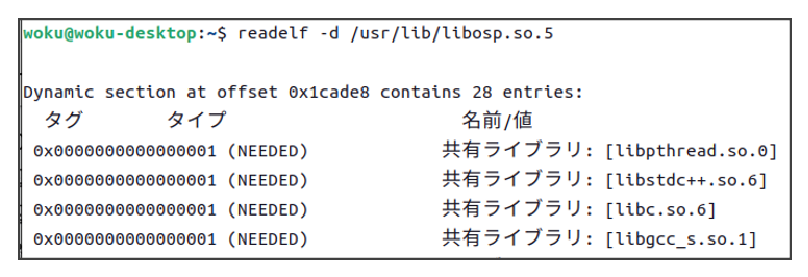
\includegraphics[width=11cm]{fig/d3.eps}
	\caption{libosp.so.5の動的セクション}
	\label{fig:d2}
\end{figure*}

\begin{figure*}[t]
	\centering
  \includegraphics[width=11cm]{fig/d4.eps}
	\caption{オブジェクトの依存関係の探索順序}
	\label{fig:d2}
\end{figure*}

\subsection{依存関係のあるオブジェクトの特定方法}

最初に依存関係を解決するオブジェクトとして,実行を行う実行ファイルがある.実行ファイルを管理するリンクマップをmain\_mapという.
main\_mapとともに,最初に依存関係を解決するオブジェクトとして,LD\_PRELOAD環境変数,-preloadオプション,/etc/ld.so.preloadファイルのいずれかで指定されたパスのオブジェクトがある.
これは,動的リンカのプリロード機能を使用して,優先的にロードさせるオブジェクトとして扱われる.プリロードを行うオブジェクトのリンクマップはpreloads配列に保存され,
依存オブジェクトの探索は,main\_map,preloadsの順で行われる.

次に,オブジェクトが依存する共有オブジェクトを特定するために,動的リンカはオブジェクトの動的セクションにあるNEEDEDエントリの値を参照する.
例えば,図3はlibosp.so.5共有オブジェクトの動的セクションの一部である.このオブジェクトが依存する共有オブジェクト名が4つのNEEDEDエントリにそれぞれ格納されていることが分かる.
NEEDEDエントリはコンパイル時に必要な共有ライブラリを特定することで作成される.


\subsection{シンボルの探索が行われるオブジェクトの順番}
図4に,シンボルの探索が行われるオブジェクトの順序決定例を示す.
初めに,実行ファイルであるmain\_map自身から探索を行い.次にpreloadsの共有オブジェクトを順に探索する.その後,main\_mapが依存するオブジェクトを幅優先で探索し,main\_mapの依存オブジェクトを全て探索した後,
preloadsの依存オブジェクトを探索していく.
main\_mapが本来依存するシンボルと同名のシンボルがpreloadsのどこかに存在した場合,シンボルの置き換えが発生するのは,この順序でシンボルテーブルの探索を行うからである.\\




\section{おわりに}
Dynamic Linker Hijackingの動的リンク段階での対策を検討するために,動的リンクの詳細な設計を調査した.
動的リンカとLinux Kernelのソースコードをもとに,実行ファイル実行ファイル実行における,動的リンカの動作範囲を明らかにした.
これにより,調査を行うべき動的リンカのソースコードと,デバッグのタイミングが特定できた.
また,範囲を特定したソースコードに対して詳細な調査を行い,シンボル解決が行われるオブジェクトの順序がどのように決まるかを明らかにした.
今後は,今回得られた知見をもとに,依存オブジェクト間に重複シンボルがある場合を検知する方法を考えたい.
共有オブジェクトの検索パスの決定方法など,動的リンカの処理内容で明らかにできていない部分に対しても調査を行なっていく.

%bibtex
\setlength\baselineskip{12pt}
{\small
	\bibliography{references}
	\bibliographystyle{ipsjunsrt}
}


\end{document}
